%%%%%%%%%%%%%%%%%%%%%%% file template.tex %%%%%%%%%%%%%%%%%%%%%%%%%
%
% This is a general template file for the LaTeX package SVJour3
% for Springer journals.          Springer Heidelberg 2010/09/16
%
% Copy it to a new file with a new name and use it as the basis
% for your article. Delete % signs as needed.
%
% This template includes a few options for different layouts and
% content for various journals. Please consult a previous issue of
% your journal as needed.
%
%%%%%%%%%%%%%%%%%%%%%%%%%%%%%%%%%%%%%%%%%%%%%%%%%%%%%%%%%%%%%%%%%%%
%
% First comes an example EPS file -- just ignore it and
% proceed on the \documentclass line
% your LaTeX will extract the file if required
%
%
\RequirePackage{fix-cm}
%
\documentclass{svjour3}                     % onecolumn (standard format)
%\documentclass[smallcondensed]{svjour3}     % onecolumn (ditto)
%\documentclass[smallextended]{svjour3}       % onecolumn (second format)
%\documentclass[twocolumn]{svjour3}          % twocolumn
%
\smartqed  % flush right qed marks, e.g. at end of proof
%
\usepackage{graphicx}
\usepackage{enumerate}
\usepackage{paralist} 
\usepackage{amsmath}
\usepackage{float}
\usepackage{booktabs}
% \usepackage{mathptmx}      % use Times fonts if available on your TeX system
%
% insert here the call for the packages your document requires
\usepackage{latexsym}
%\usepackage{hyperref}
\usepackage{algorithm}
\usepackage{algorithmic}
%\usepackage{algpseudocode}
% etc.
%
% please place your own definitions here and don't use \def but
% \newcommand{}{}
%
% Insert the name of "your journal" with
% \journalname{myjournal}
%
\renewcommand{\algorithmicrequire}{\textbf{Input:}}
\renewcommand{\algorithmicensure}{\textbf{Output:}}

\begin{document}

\title{A Cost-sensitive Algorithm with Local and Global Consistency
\thanks{Supported by the Natural Science Foundation of China under Grant No. 61471083, 61300017, the Fundamental Research Funds for Central Universities (DUT15QY28)}}
\subtitle{}

%\titlerunning{Short form of title}        % if too long for running head

\author{Weifeng Sun       \and
        Jianli Sun %etc.
}

%\authorrunning{Short form of author list} % if too long for running head

\institute{W. Sun \at
              School of Software, Dalian University of Technology \\
              DaLian, 116620 - China \\
              \email{}           %  \\
%             \emph{Present address:} of F. Author  %  if needed
           \and
           J. Sun \at
           School of Software, Dalian University of Technology\\
           DaLian, 116620 - China\\
           \email{sjl\_dlut@163.com}
}

\date{Received: date / Accepted: date}

% The correct dates will be entered by the editor


\maketitle
\begin{abstract}
Assuming that misclassification costs among different categories are equal, traditional graph based semi-supervised classification algorithms pursuit high classification accuracy. However, in many practical problems, misclassifying one category as another always leads to higher (or lower) cost than that in turn, such that, higher classification accuracy generally not means lower cost, which is more important in these problems. Cost-sensitive classification methods enable classifiers to pay more attention to data samples with higher cost, and then attempt to get lower cost by ensuring higher classification accuracy of the category with higher cost. In this paper, we bring cost sensitivity to local and global consistency (LGC) classifiers, and propose the CS-LGC (cost-sensitive LGC) methods, which can make better use of semi-supervised classification algorithms, and ensure high classification accuracy on the basis of reducing overall cost. At the same time, since the improved algorithm may bring some problems due to unbalanced data, we introduce a SMOTE algorithm for further optimization. Experimental results of bank loan and diagnosis problems verify the effectiveness of CS-LGC.
\keywords{Graph based semi-supervised classification \and Cost-sensitive \and Rescale \and SMOTE}
% \PACS{PACS code1 \and PACS code2 \and more}
% \subclass{MSC code1 \and MSC code2 \and more}
\end{abstract}

\section{Introduction}
\label{intro}

%Text with citations  and \cite{urner2011access} \cite{zhou2010semi} \cite{zhu2009introduction} \cite{budvytis2010label} \cite{zhu2003semi} \cite{zhou2004learning} \cite{gao2011active} \cite{elkan2001foundations} \cite{zhou2010multi} \cite{domingos1999metacost} \cite{khoshgoftaar2011comparing} \cite{fan1999adacost} \cite{jin2010multi} \cite{qin2008cost} \cite{liu2006influence} \cite{seiffert2008comparative} \cite{bache2013uci} \cite{germandata} \cite{mangasarian1990pattern}

Recently, machine learning classification algorithms have achieved sound development in multimedia identification, health care, finance, and many other applications. Among them, Graph-based Semi-Supervised Classification based on perfect graph theory, which is relatively straightforward and easy to understand, has become one of the hottest research focuses. This method can make better use of the information from labeled data and a great deal of data distribution information mined from unlabeled data, then solves the problem of the less labeled data and the huge labeling costs.

High classification accuracy is the target of GSSC algorithm, which assumes that the cost of misclassification among different categories is the same. However, in many practical problems,  the costs of category classifications is different, especially in the fields of medical service, finance and network security and so on.

For example, in the bank loan problem, banks decide whether to approve the loan based on the loan applicants' personal information, which can be viewed as a binary classification problem. In the process of approving a bank loan, the cost of approving an applicant who is unable to repay the loan is much greater than that of approving an applicant who can repay the loan. Similarly, in the disease diagnosis, the cost of misdiagnose unhealthy patients as healthy is much greater than that of misdiagnose healthy patients as unhealthy. When the cost differences are inconsistent among different categories, a classifier paying more attention to the accuracy of higher cost classification problem is more practical than those treat all categories equally.
%Text with citations  and \cite{urner2011access} \cite{zhou2010semi} \cite{zhu2009introduction} \cite{budvytis2010label} \cite{zhu2003semi} \cite{zhou2004learning} \cite{gao2011active} \cite{elkan2001foundations} \cite{zhou2010multi} \cite{domingos1999metacost} \cite{khoshgoftaar2011comparing} \cite{fan1999adacost} \cite{jin2010multi} \cite{qin2008cost} \cite{liu2006influence} \cite{seiffert2008comparative} \cite{bache2013uci} \cite{germandata}

Cost-sensitive learning method \cite{gao2011active,elkan2001foundations,zhou2010multi,domingos1999metacost,fan1999adacost} takes the inconsistencies of cost among categories into account to lower the overall cost for the target. This method defines the static cost matrix to make classifiers pay more concern to the sample data with higher cost, and improves classification accuracy of higher-cost category. In the semi-supervised classification problems, labels account for a small portion of the data and most data are unlabeled. Actually, the traditional semi-supervised classification treats all categories equally, which cannot guarantee a lower overall cost. Meanwhile, cost-sensitive learning may arise less fit due to limited data set of tags, which could lead to lower classifier accuracy and weaker generalization ability. Besides, in the semi-supervised learning, we often encounter the situation called uneven data problem, in which different types of samples have different numbers of labeled data.

In summary, researches on cost-sensitive semi-supervised classification algorithms for unbalanced datasets are of great significance to the development of finance, medical fields, network security and many other areas.

\section{Related Work}
The effectiveness of semi-supervised learning algorithm depends on the three assumptions: manifold hypothesis\cite{urner2011access,zhou2010semi}, mlustering hypothesis and smoothness hypothesis. GSSC based on manifold hypothesis builds a figure to describe the data, as well as the relationship between the data. In this figure, nodes represent the data samples while edges with weight represent the relationships between samples. At the same time, the larger the weight is, the higher the similarity of the samples have. The process that GSSC classifiers assign labels to unlabeled data is the process of label propagation in the figure. Label Propagation Algorithm Budyytis et al. proposed in \cite{budvytis2010label}  can calculate the probability of transfer among tag data by the topology and the similarity between the samples in figure, and make a label transfer by combining node out-degree. A method of Gaussian fields and harmonic functions proposed by Zhu et al. in \cite{zhu2003semi} that make discrete prediction function slack to become continuous prediction function considers the transfer probability samples fully and have a label transfer in $k$-connection diagram. Local and global consistency, LGC proposed by Zhou et al. in the \cite{zhou2004learning} introduced clustering hypothesis and had a label transfer by using local and global consistency. LGC algorithm gives a rigorous mathematical logic derivation and proves the convergence. However, these related works never consider the problem of inconsistent classification cost.

Cost-sensitive learning method is an effective way to solve the problem of the inconsistency of costs. Cost-sensitive learning method introduces cost matrix to describe the inconsistency of costs among categories and get global minimum cost. The cost-sensitive classification methods can be divided into two categories: Rescale and Reweight, depending on the representations of cost. In the method of Rescale, differences in cost are described as differences among the numbers of samples, such as Cost-sensitive sampling\cite{gao2011active}, Rebalance\cite{elkan2001foundations} and Rescale new\cite{zhou2010multi} etc. This method constructs different sample data sets according to the difference in costs which make classifiers' decision face prefer samples with more costly category. Reweight method describes differences in costs by differences in weight among samples of different types. In the method of Reweight, samples with costly category have a higher weight, which make a greater impact to classifier. MetaCost\cite{domingos1999metacost} is a typical representative of such Reweight methods. MetaCost based on Bayesian risk theory adds the cost of the sensitive nature for Non-cost-sensitive classification algorithm by using bagging\cite{khoshgoftaar2011comparing}.

AdaBoost algorithm was proposed in\cite{jin2010multi} which offers the possibility for multiple weak classifiers aggregating into a global strong classifier. AdaCost method\cite{fan1999adacost} was proposed as a cost-sensitive classification algorithm based on AdaBoost. AdaCost is based on the Reweight at the same time, and introduces cost performance function for classifiers by heuristic strategy. AdaCost forces classifier to pay more attention to costly samples, hence it shows some advantages in cost-sensitive classification problems. However, cost performance function introduced in the theoretical analysis have not been verified and damages the most important characteristics of Boosting,  which makes the algorithm not converge to the Bayesian decision. Qin etc. in \cite{qin2008cost} did try to combine semi-supervised classification algorithms with cost-sensitive learning methods, and improved classical EM algorithm by introducing misclassification cost in the process of probability assessment.

In this paper, advantages of many unlabeled data are fully taken. We use the method of Rescale to describe cost inconsistency and introduce cost-sensitive nature for LGC algorithm classic semi-supervised classification algorithm. We propose a cost-sensitive LGC method—CS-LGC algorithm. At the same time, we take the impact caused by unbalanced data into account for CS-LGC algorithm, improve the CS-LGC algorithm by proposing the average similarity concept and introduce SMOTE algorithm. The main contribution of this paper is as follows:
\begin{enumerate}[(1)]
  \item Introduce cost-sensitive nature for LGC algorithm, and propose cost-sensitive LGC algorithm;
  \item Propose CSS-LGC algorithm. We take the impact caused by unbalanced data into account for CS-LGC algorithm, and we propose optimized CS-LGC algorithm—CSS-LGC algorithm.
  \item Analyze the experimental threshold, and verify the rationality of the threshold. 
  \item Demonstrate the effectiveness of the algorithm by experiment on German Credit Data Set and Breast Cancer Data Set.
\end{enumerate}

\section{CSS-LGC Algorithm}
\subsection{Problem Definition}
Many problems can be described as binary classification problems (multiple class classification problems can be split into multiple binary classification problem), so this paper simply discusses binary classification problem. The two classes can be defined as positive class whose sample number is denoted as ${N_ + }$, and negative class with the sample number denoted as ${N_ - }$. We further assume $C_{-+}$, the cost that a sample in negative class is classified into positive class is much bigger than that in turn.${\rm{X}} = \left\{ {{x_1},{x_2}, \ldots ,{x_l},{x_{l + 1}}, \ldots ,{x_{l + u}}} \right\}$ is a set of data samples, where $l$ is the number of labeled data, and $\left\{ {{x_1},{x_2}, \ldots ,{x_l}} \right\}$ forms the initial labeled data sets. $u$ represents the number of unlabeled data, thus $U=l+u$ denotes the total number of samples. ${x_i}$ is a multidimensional vector of the $i$-th data with several features, which can be viewed as a point in higher dimensional space. Those data points and their relationships can be described by a fully connected graph $G = \left( {V,E} \right)$, where $V \in {R^{N \times P}}$ represents the vertex set of $G$, $P$ is the feature value of each data sample. we have $V = X$ here, and $E$ is the edge set of $G$. Similarity among data points is important in classification, clustering and other machine learning fields. In LGC algorithm, similarity among data points is described by weight matrix $W \in {R^{N \times N}}$. Labeled data information is described by labeled information matrix $Y \in {L^{N \times 2}}$, where $L = \left\{ { + 1, - 1} \right\}$. If data $i$ belongs to category $j$, then ${Y_{ij}} = 1$, otherwise ${Y_{ij}} = 0$. The initial labeled information matrix only has a little labeled information.

Liu and Zhou mentioned that the cost of misclassification can be standardized in \cite{liu2006influence}, which will not affect the best decision when calculation is simplified. In this paper, we let ${c_{ +  - }} = 1$, so  ${c_{ - + }}$ is a real number larger than $1$. In order to make semi-supervised classifier cost sensitive, We introduce sample cost information for the initial label matrix, denote cost difference using different initial labeled information volumes, and process the initial label matrix as Formula \ref{formula1} shows:
\begin{equation} \label{formula1}
YN_{.i} = {T_0} \circ {Y_{ \cdot i}} 
\end{equation}
${N_{.i}}$ indicates the $i$-th column of the processed initial label matrix. $\circ $ indicates Adama product. $T_0$ indicates the cost of sample data at the initial time. In addition
\begin{equation}
{T_0}({x_i})=
  \begin{cases}
  1/{N_ +}& \mbox{if } x_i \mbox{ is positive class} \\
  {C_{-+}}/{N_ - } & \mbox{if } x_i \mbox{ is negative class}  
  \end{cases}
\end{equation}

CS-LGC method is designed to classify all data samples using the information of graph $G$ with unknown $Y$ and ${T_0}$. Our goal is to ensure unlabeled data to obtain class label as much as
possible without changing the information of labeled data, and at the same time, minimize the global  classification cost without damaging classification accuracy.
\subsection{Algorithm Process}
CS-LGC method is a boosting process that trains semi-supervised classifiers in each iteration and update labeled data set based on the performance of the classifiers.
At the initial time, semi-supervised classifier $h_0$ is trained using traditional LGC algorithm
according to preprocessed initial label matrix, and we further calculate error rate by Formula \ref{formula3}.
\begin{equation} \label{formula3}
  {\varepsilon _0} = \frac{{\mathop \sum \nolimits_{i = 1}^N I\left( {{y_{i,{h_0}\left( {{x_i}} \right)}} = 0} \right)}}{N}
\end{equation}
Here $I$ is a binary function, whose value is $1$ if conditions are satisfied, or is 0 else. ${h_0}\left( {{x_i}} \right)$ shows classification results for $x_i$ at the initial time. Then according to the AdaBoost algorithm, cost information of misclassified samples increases while cost information of correctly classified samples decreases following Formula \ref{formula4},
\begin{equation} \label{formula4}
  {T_{t + 1}}\left( {{x_i}} \right) = \frac{{{T_t}\left( {{x_i}} \right)}}{{{Z_t}}} \times 
  \begin{cases}
    {{e^{ - {\alpha_t}}}} & \text{if } {{y_{i,{h_t}\left( {{x_i}} \right)}} = 1} \\
    {{e^{{\alpha_t}}}} & \text{if } {{y_{i,{h_t}\left( {{x_i}} \right)}} = 0}
  \end{cases}
\end{equation}
where ${T_{t + 1}}$ represents the updated cost matrix, and
\begin{equation}
  {Z_t} = \mathop \sum \limits_{i = 1}^N {T_t}\left( {{x_i}} \right) \times 
  \begin{cases}
     {{e^{ - {\alpha_t}}}} & \text{if } {{y_{i,{h_t}\left( {{x_i}} \right)}} = 1} \\
     {{e^{{\alpha_t}}}} & \text{if } {{y_{i,{h_t}\left( {{x_i}} \right)}} = 0}   
  \end{cases}
\end{equation}
where ${\alpha _t}$ represents the weight of classifier $h_t$í±¡ in the final global classification at time $t$, and can be calculated by
\begin{equation}
  {\alpha _t} = \ln \left( {\frac{{1 - {\varepsilon _t}}}{{{\varepsilon _t}}}} \right)
\end{equation}

The main objective of Cost-sensitive classifier is to minimize global classification. To avoid the
impact of data set scale on the results, the calculation of global cost in our model use the mean cost method brought by Seiffert et al\cite{seiffert2008comparative}. Since we have to standardize classification cost of our model, the corresponding mean cost needs to be updated according to Formula \ref{formula7}:
\begin{equation} \label{formula7}
  PEC=\frac{{\# {f_{pos}} + \# {f_{neg}} \cdot {C_{ -  + }}}}{{\# {t_{pos}} + \# {t_{neg}} + \# {f_{pos}} + \# {f_{neg}}}}
\end{equation}
where $PEC$ denotes the average cost of classifiers, ${\# {t_{pos}}}$ and ${\# {f_{pos}}}$  denote the number of positive class samples classified correctly and classified incorrectly respectively. ${\# {t_{neg}}}$ and ${\# {f_{neg}}}$ represent the corresponding information of negative class. The global cost we refer to here that is indeed the average cost. From Formula \ref{formula7} we can see that the correct classified samples does not increase the global cost. 

Next, we update the label matrix $YN$ according to Rescale Method. Specifically, when the cost of $x_i$ increases, means there is a wrong classification. Then a certain number of data that have the highest similarity with $x_i$ are chosen from unlabeled data set and added into labeled data set. The class and cost information of the newly added data are the same with $x_i$. On the contrary, when sample data $x_i$'s cost decreases, and the decreasing range is larger than the threshold $ts$, then we will remove $x_i$ and its label information from the labeled data set.

After then, we train the classifier of the next time according to updated label matrix and repeat the process until the global cost difference between two training time step is less than a certain
threshold. Finally, a global classifier can be obtained by the way of weighted voting.
\begin{equation}
  {Y_{final}}\left( {{x_i}} \right) = sign\left( {\mathop \sum \limits_{j = 1}^M {\alpha _j}{h_j}\left( {{x_i}} \right)} \right)
\end{equation}
Here $M$ denote the number of classifier when the iteration ends. 

In summary, the process of CS-LGC method is shown in Algorithm \ref{algo:cs-lgc}:
\begin{algorithm}[h] 
  \begin{algorithmic}[1]
    \REQUIRE{data set $X$, the initial label matrix $Y$}
    \STATE{add cost information for the initial label matrix according to Formula \ref{formula1}}
    \WHILE{$\Delta PEC \ge threshold$}
      \STATE{train LGC semi-supervised classifier}
      \STATE{update the cost matrix by Formal \ref{formula4} according to the result}
      \STATE{update labeled data set applying Rescale Method}
      \STATE{update the initial label matrix according to Formula \ref{formula1}}
    \ENDWHILE
    \ENSURE{${{\rm{Y}}_{final}}({x_i}) = sign(\sum\limits_{j = 1}^M {{\alpha _j}{h_j}({x_i})} )$
  , $  PEC=\frac{{\# {f_{pos}} + \# {f_{neg}} \cdot {C_{ -  + }}}}{{\# {t_{pos}} + \# {t_{neg}} + \# {f_{pos}} + \# {f_{neg}}}}$ }
  \end{algorithmic}
  \caption{CS-LGC}
  \label{algo:cs-lgc}
\end{algorithm} 

% \subsection{The convergence of the algorithm}
% \begin{proof}
%  The convergence of the CS-LGC algorithm depends on the convergence of the LGC, and whether the cost of the sample data by wrong classification has an upper limit. For ease of reading, we use $c_i$ ($\frac{1}{{{N_ + }}}$ or $\frac{{{C_{ -  + }}}}{{{N_ - }}}$ or $0$) to denote the cost of sample $i$, and $y_i$(-1 or +1) to denote the real label of sample $i$.

% Zhou gives the evaluation function based on FIG of the semi-supervised classification algorithm in \cite{zhou2004learning}, which is usual composed of smooth function and loss function. According to
% extremum condition acquired by evaluation function as well as recursion formula of LGC algorithm, Zhou deduces the convergence formula (Formula \ref{formula9}) of LGC algorithm, then proves the convergence of LGC algorithm.
% \begin{equation}\label{formula9}
%   F = {(I - \beta S)^{ - 1}}Y
% \end{equation}
% Here $F$ is the final classification function, $\beta  \in \left( {0,1} \right)$, $S$ is a symmetric matrix, and
% \begin{equation}
%   {\text{S}} = {D^{ - 1/2}}W{D^{ - 1/2}}
% \end{equation}
% where D is a diagonal matrix, whose diagonal elements is the sums of elements of corresponding row vectors in the weight matrix $W$.

% For the cost matrix of CS-LGC algorithm, Formula \ref{formula4} can be rewritten as
% \begin{equation}
%   \begin{aligned}
%     {T_{t + 1}}(i) &= {T_t}(i)\frac{{{e^{ - {\alpha _t}{y_i}{h_t}({x_i})}}}}{{{Z_t}}}\\
%     &= {T_1}(i)\frac{{{e^{ - {y_i}\sum\limits_{j = 1}^M {{\alpha _j}{h_j}({x_i})} }}}}{{\prod\limits_{j = 1}^S {{Z_j}} }}
%   \end{aligned}
% \end{equation}
% Because of $\sum\limits_{i = 1}^N {{T_{t + 1}}(i)}  = 1$, we have
% \begin{equation}
%     \prod\limits_{j = 1}^M {{Z_j}}  = \frac{1}{{{N_ + }}}\sum\limits_{i = 1}^{{N_ + }} {{e^{ - {y_i}\sum\limits_{j = 1}^M {{\alpha _j}{h_j}({x_i})} }}}  + \frac{{{C_{ -  + }}}}{{{N_ - }}}\sum\limits_{k = 1}^{{N_ - }} {{e^{ - {y_{\text{k}}}\sum\limits_{j = 1}^M {{\alpha _j}{h_j}({x_k})} }}} 
% \end{equation}
% where $x_i$ denotes the positive class sample, and $x_k$ denotes the negative class sample.

% In the binary classification problem, the label of data is either -1 or +1, and when ${y_i} \ne {Y_{final}}({x_i})$, ${y_i}{Y_{final}}({x_i}) \le 0$ holds, then we have ${e^{ - {y_i}{Y_{final}}({x_i})}} \ge 1$. The global cost of the classification can be calculated by Formal \ref{formula13},
% \begin{equation} \label{formula13}
%   \begin{aligned}
%   E &= \sum\limits_{j = 1}^N {c_j}
%   \begin{cases}
%   1 & \mbox{if } {y_j} \ne {Y_{final}}({x_j}) \\
%   0 &  \mbox{else }
%   \end{cases} \\
%   &\le \sum\limits_{j = 1}^N {{c_j}{e^{ - {y_j}{Y_{final}}({x_j})}}}  \\
%   &= \sum\limits_{j = 1}^N {{c_j}\prod\limits_{i = 1}^M {{Z_i}} \frac{{{T_M}({x_j})}}{{{T_0}({x_j})}}} \\
%   &= d\prod\limits_{i = 1}^M {{Z_i}} 
%   \end{aligned}
% \end{equation}
% there $d$ denotes the sum of all the data samples' costs initially. 

% In conclusion, when the cost matrix is decided, LGC algorithm will converge to Formal \ref{formula9}, and the upper bound of cost matrix does exist (Formal \ref{formula13}), thus CS-LGC algorithm can converge.
% \qed
% \end{proof}

\section{Improved CS-LGC Algorithm: CSS-LGC}
\subsection{Defect Analysis of CS-LGC Algorithm}
 According to the updated cost matrix, $Q$ data need selecting from the labeled data to join the negative class. However, it turns out that the number of the unlabeled data is smaller than $Q$  after calculating the average similarly. The average similarity is more close to either positive class or negative class. That is the problem we often encounter with unbalanced data sets, at this time this situation may come: classification precision appears fluctuant, leading to unstable performance. In response to this problem of unbalanced data sets, we introduce in SMOTE algorithm, i.e. using the method of synthetic artificial virtual data to solve the serious problem of unbalanced data sets, so as to solve the problem of unstable performance of the classifier.

\subsection{CSS-LGC Algorithm Process}
 SMOTE algorithm generates virtual data through a synthetic way. For each minority category sample, the method looks for its $k$ samples with the highest similarity. Then Upward sampling method is applied. If the amount of upward sampling samples is set as $N$, it randomly selects $N$ samples from all $k$ samples, which can be represented as ${x_i}\left( {i = 1,2, \ldots ,N} \right)$, then conducts the linear interpolation between minority class $x$ and $x_i$. Next, it constructs new minority samples ${p_1},{p_2},...,{p_N}$ and 
 \begin{equation}
  {p_i} = x + rand(0,1)*({x_i} - x), \quad i = 1,2,\ldots,N
 \end{equation}

 The process of CSS-LGC algorithms is roughly same with CS-LGC, except the difference when CSS-LGC
algorithm uses Rescale to update labeled data sets. 

In the CSS-LGC algorithm, after updating the cost matrix, Rescale is applied to update label matrix, then, it adds SMOTE method and optimizes the overall process of updating the label matrix. The
specific implementation process is as follows:
\begin{enumerate}[1)]
  \item According to the change of cost matrix before and after the update, we determine the amount of required unlabeled data chosen in each category.
  \item First of all, we get average similarity respectively for samples that have been marked as positive class from the remaining unlabeled data. Then we get the average similarity between the samples of each unlabeled and all samples that have been marked as positive class, denote them as ${p_1},{p_2},\ldots ,{p_u}$, where $u$ represents the number of unlabeled samples. In the same way,  we use all unlabeled data to get an average similarity for the samples that has been marked as negative class, which denoted as $p_1^\prime ,p_2^\prime , \ldots ,p_u^\prime $. Here ${p_1},{p_2},\ldots ,{p_u}$ and $p_1^\prime ,p_2^\prime , \ldots ,p_u^\prime $ are respectively calculated by Formula \ref{formula15} and Formula \ref{formula16},
  \begin{equation} \label{formula15}
    {p_j} = (\mathop \sum \limits_{i = 1,{{\text{Y}}_{i1}}{\text{ =   + }}1}^l {w_{\left( {l + j} \right)i}})/{N_ + },\quad j = 1,2,\ldots,u.
  \end{equation}
  \begin{equation} \label{formula16}
  p_j^\prime  = (\mathop \sum \limits_{i = 1,{{\text{Y}}_{i1}}{\text{ =   - }}1}^l {w_{\left( {l + j} \right)i}})/{N_ - },\quad j = 1,2,\ldots,u.
  \end{equation}
  where $N_+$ and $N_-$, respectively denote the number of the positive and negative samples in the data that have been marked, $Y$ is the label matrix, and $W$ is the weight matrix.
  \item According to select unlabeled data, two conditions need meeting: first, the average similarity
of unlabeled data must be closer to the class which will be marked as; Second, data with average similarity closer to this category unlabeled data should be chosen in accordance with descending order of average similarity and the number of unlabeled data to select calculated in the first step. At this time, it will have two cases:
\begin{enumerate}[a)]
 \item The number of average similarity of unlabeled data closer to this class which will be marked as is enough, that is to say, we can find out enough samples from unlabeled data for this class.
 \item There are few samples with average similarity closer to the class in the unlabeled data, namely, the number of unlabeled data with similarity to be marked in this class is  littler than the other class, or only a small portion of data are more similar to this class.
\end{enumerate}
If this is the first case, after completing marking the selected unlabeled data, we can simply exit the Rescale process, then update the initial label matrix In line with formula \ref{formula1} and go on with the following study. Otherwise, as the second case occurs, we jump to the fourth step to process. \label{step3}

\item After making some artificial virtual data using SMOTE method, we jump to the second step, and continue conduct, until the number of artificially manufactured unlabeled data is more closer to
the number that this class need to be marked, and when the number the number is abundant, jump to the process of the first case in step \ref{step3}.

\end{enumerate}

In the process of above, when synthesizing artificially data by using SMOTE algorithm for each minority class that need unlabeled data, instead of applying the method of upward sampling, our solution is to determine the number of unlabeled data to select according to the cost ratio of before  to after updating. For instance, when the cost ratio is $r$($r>1$), then the number of unlabeled data to select is $r-1$. At this time, we need to choose $r-1$ samples from the $k$ unlabeled samples with the highest similarity and do linear interpolation with minority class samples.

Through improving Rescale process of the CS-LGC algorithm, we solve the defection of classification errors, which may accumulate in the unbalanced dataset and enhance the stability of classifiers' performance.

\subsection{Performance Analysis of CSS-LGC Algorithm}
The increased time complexity by introducing cost sensitive feature to semi-supervised classification algorithm based on graph is mainly reflected in the process of boosting and updating cost matrix.

The aim of updating the cost matrix is to update the labeled data set, including adding new labeled data and deleting existing labeled data. The adding operation has a relatively higher time complexity, which reaches $O(l \cdot n\lg n) < O({n^2}) $, where $l$ is the number of labeled data. Besides, choosing the unlabeled data with high similarity, which can be seen as a sorting, has the time complexity of $O(n\lg n)$. The time complexity of boosting process is $O(M \cdot {n^3})$ ,  the time complexity of base-classifier LGC algorithm reaching $O({n^3})$ included and $M$ represents the number of base-classifiers. The time complexity of CS-LGC algorithm depends on the number of base-classifiers denoted as $M$. From the following experiments, we can know, in the problem of bank loan, disease diagnosis etc., the number of convergences in CS-LGC is not sufficient to make the classifier time complexity increased by one order of magnitude.

\section{Experimental Results and Analysis}
\subsection{Data Introduction and Preprocessing}
We choose bank loans and disease diagnosis, whose misclassification costs are inconsistent, to
test our CS-LGC and CSS-LGC algorithm. Since the fact that CS-LGC is the improvement of LGC, we will verify whether CS-LGC’s global cost will be reduced and whether its accuracy will be lowered compared with LGC. In addition, CS-LGC is a cost-sensitive classification method, so we will compare it with a traditional cost-sensitive algorithm, AdaCost algorithm, to see the performance difference between two algorithms.

Cost-sensitive learning focuses more on sample data of high cost, so in this paper, we implement three experiments to verity the properties of CS-LGC and CSS-LGC:
\begin{inparaenum}[(1)]
  \item the classification accuracy of high cost category changes with the labeled data;
  \item the global classification accuracy changes with the labeled data;
  \item the global cost changes with labeled data.
\end{inparaenum}

German Credit Data Set\cite{germandata}, which describes the information of bank loan applicants and whether the information of the relevant loan application is approved, was provided by Professor Hans Hofmann Et al. The data set collected 1000 loan applicants' information, including current deposit, borrowing time, fixed asset, working condition as well as whether they have guarantee and so on. There are 20 characteristic attributes in all. Finally, the applications of 700 person were approved while the other 300 applications weren't. We define the people who got the approvals as positive class, and those who did not as the negative class, then set ${C_{ +  - }} = 1$, ${C_{ -  + }} = 5$, and initialize the cost of CS-LGC after standardizing process. Different features will represent in different value ranges, such as applicants' genders only have 0 and 1, two small value, while borrowing time could reach 48 (months) or even much larger. To eliminate this difference, feature values  of characteristics for the applicants should be linear normalized as Formula \ref{formula17}.
\begin{equation} \label{formula17}
  {x_{ij}}' = \frac{{{x_{ij}} - {x_{i\min }}}}{{{x_{i\max }} - {x_{i\min }}}}
\end{equation}
${x_{ij}}'$ denotes the results of the $j$-th attribute value of the $i$-th applicant after normalization, ${{x_{i\max }}}$ and ${{x_{i\min }}}$ respectively denote the maximum and minimum value in all attribute values of applicant $i$.

Breast Cancer Data Set\cite{Mangasarian90} was provided by the Professor Mangasarian and Wolberg of University of Wisconsin. It offers the feature information of breast cancer patients in the University of Wisconsin and the diagnosis of their disease (benign or malignant). This data set collected 10 attributes of 699 patients, such as the uniformity of patients' cell size. There are 458 cases diagnosed as benign, the other 241 cases as malignant. We treat benign patients as positive class, and malignant as negative class. Since the data set does not show information on the cost of misclassification, the ratio of the numbers of two classes whose samples are normalized will be defined as cost, which can be written as ${C_{ +  - }} = 1$ and ${C_{ -  + }} = 1.9$. We remove the attributes which have little things to do with the diagnosis, such as ID number, all other attributes range from 1 to 10, without the necessity of normalization. However, 16 records have some missing attributes, including 13 positive samples and 3 negative samples. After removing those invalid records , the ratio of positive class to negative is $445:328$.

\subsection{Experimental Setting}
The labeled data in this experiment are randomly selected from the data set. In order to observe the influence of the number of labeled data on classification results, We choose $10\%, 20\% \ldots 90\%$ ( increased by 10\% at one time) data from the whole data set as the labeled. Then we design and run the experiments on Matlab R2010a. When updating the labeled data set following Rescale method, the cost of samples decrease by more than 50\%, those samples will be removed from the labeled data set, that is to say, we set $ts = 50\% $. The termination criterion for the iteration of CS-LGC method is that the difference of global costs between the latest two iteration, which is the value of $threshold$, reaches 10\% or less. The experimental settings of LGC method, Adacost algorithm and CS-LGC algorithm are the same as the CSS-LGC method. All the experimental data shown following are the average results of 50 times repeated experiments.

\subsection{Threshold Discussion}
These two thresholds need to be set in CS-LGC and CSS-LGC algorithm: The first one is $ts$, the decent degree threshold of sample data $x_i$'s cost. When the cost of $x_i$ decreases more than $ts$, it will be deleted from the labeled data set. Another is $threshold$, the global cost difference threshold of classifier between two iterations, that is to say, When the global cost difference between two consecutive iterations is less than the $threshold$ value, the classifier will stop iteration. Here, we only discuss about the $threshold$ of CSS-LGC algorithm.

$threshold$ is set as 10\% of the initial global cost.we verify the selection of the two thresholds of CSS-LGC using German Credit Data Set.

\subsubsection{$ts$}
From Table. \ref{tab:ts} we can see when $ts$ grows up to 50\%, the global cost begins to be stable. In
\ref{subsec:exp1} and \ref{subsec:exp2} of this paper, we set $ts=50\%$.

 % Table generated by Excel2LaTeX from sheet 'Sheet1'
\begin{table}[htbp]
  \centering
    \begin{tabular}{c c c c}
    \toprule
    $ts$  & Negative classification accuracy  &  Global classification accuracy & Global cost \\
    \midrule
    0.05  & 0.546 & 0.7985 & 0.82205 \\
    0.1   & 0.6876 & 0.8035 & 0.60615 \\
    0.15  & 0.7946 & 0.8274 & 0.42896 \\
    0.2   & 0.8546 & 0.8293 & 0.33755 \\
    0.25  & 0.8937 & 0.8305 & 0.27675 \\
    0.3   & 0.9254 & 0.8327 & 0.22906 \\
    0.35  & 0.9348 & 0.8346 & 0.21394 \\
    0.4   & 0.9365 & 0.8348 & 0.21102 \\
    0.45  & 0.9367 & 0.8349 & 0.21052 \\
    0.5   & 0.946 & 0.835 & 0.1965 \\
    0.55  & 0.9463 & 0.8352 & 0.19591 \\
    0.6   & 0.9464 & 0.8352 & 0.19576 \\
    0.65  & 0.9465 & 0.8353 & 0.19554 \\
    0.7   & 0.9465 & 0.8353 & 0.19554 \\
    0.75  & 0.9465 & 0.8353 & 0.19554 \\
    0.8   & 0.9465 & 0.8353 & 0.19554 \\
    0.85  & 0.9465 & 0.8353 & 0.19554 \\
    0.9   & 0.9465 & 0.8353 & 0.19554 \\
    0.95  & 0.9465 & 0.8353 & 0.19554 \\
    1     & 0.9465 & 0.8353 & 0.19554 \\
    \bottomrule
    \end{tabular}%
  \caption{Impact and Analysis Table with $ts$} \label{tab:ts}%
\end{table}%

\subsubsection{$threshold$}
In the above paper, $threshold$ is 10. Two reasons support the setting: on the one hand, when it is 10,
precision and the global cost are still within an acceptable range; On the other hand, although the corresponding results of threshold set as 6,7,8,9 are better than 10, they take much more time and converges slower.


\begin{table}[htbp]
  \centering
    \begin{tabular}{cccc}
    \toprule
    $threshold$ & Negative class classification accuracy & Global classification accuracy & Global cost \\
    \midrule
    6     & 0.9546 & 0.85  & 0.1731 \\
    7     & 0.95186 & 0.845 & 0.18071 \\
    8     & 0.9486 & 0.8425 & 0.18735 \\
    9     & 0.947 & 0.839 & 0.1922 \\
    10    & 0.942 & 0.835 & 0.2025 \\
    11    & 0.935 & 0.83  & 0.2165 \\
    12    & 0.923 & 0.82752 & 0.23624 \\
    13    & 0.908 & 0.8247 & 0.26071 \\
    14    & 0.8967 & 0.8189 & 0.28172 \\
    15    & 0.8886 & 0.8135 & 0.29765 \\
    \bottomrule
    \end{tabular}
    \caption{Impact and Analysis Table with $threshold$}
  \label{tab:threshold}
\end{table}

\subsection{German Credit Data Set}\label{subsec:exp1}

In the loan application problem, approving the applicants that should not have been approved will result in higher cost, so we set those who cannot get approved as high-cost class (negative class). Fig. \ref{fig1} to Fig. \ref{fig3} show the high-cost class classification accuracy, global classification accuracy and global cost variation curves of the three algorithms (LGC, CS-LGC and AdaCost algorithms) when the data scale increase from only 10\% to 90\% of the total data volume respectively.
\begin{figure}[H]
\begin{minipage}[t]{.5\textwidth}
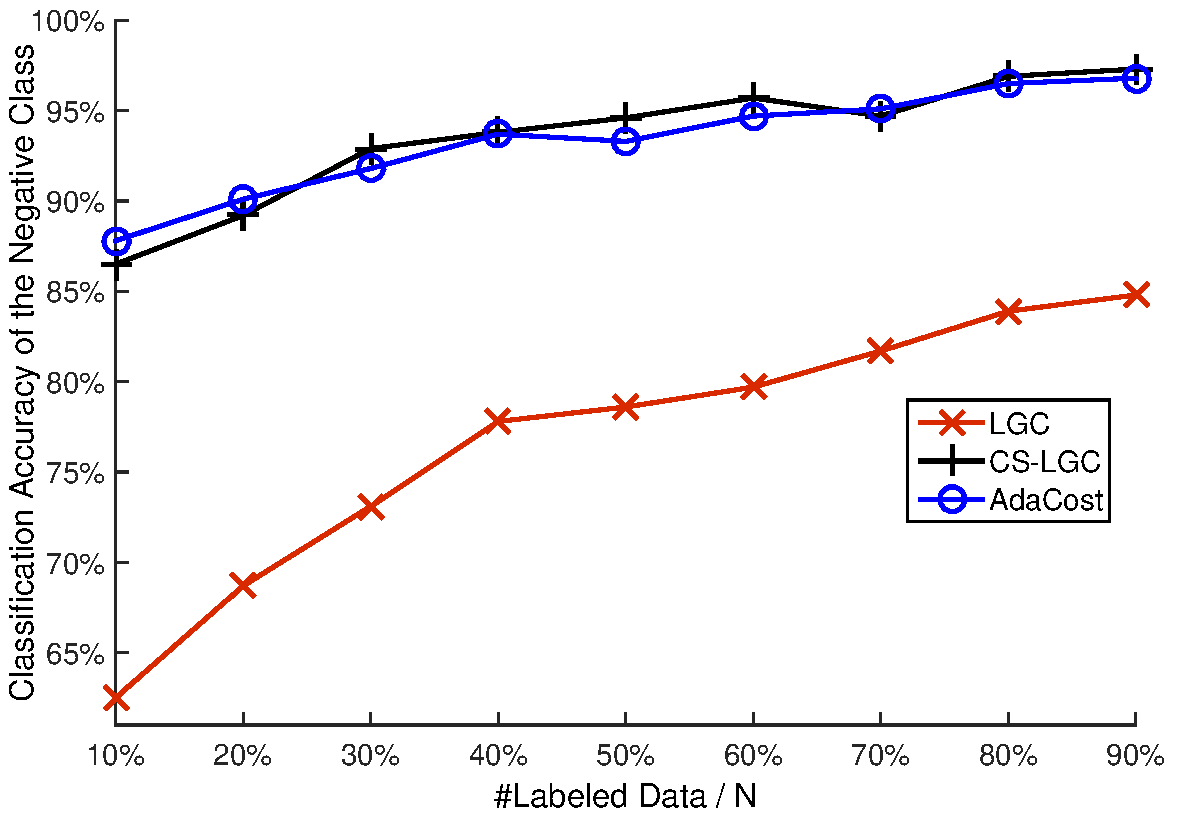
\includegraphics[width=\textwidth]{plot/fig1.pdf}
\caption{Classification Accuracy of High-cost Class Samples} \label{fig1}
\end{minipage}
\begin{minipage}[t]{.5\textwidth}
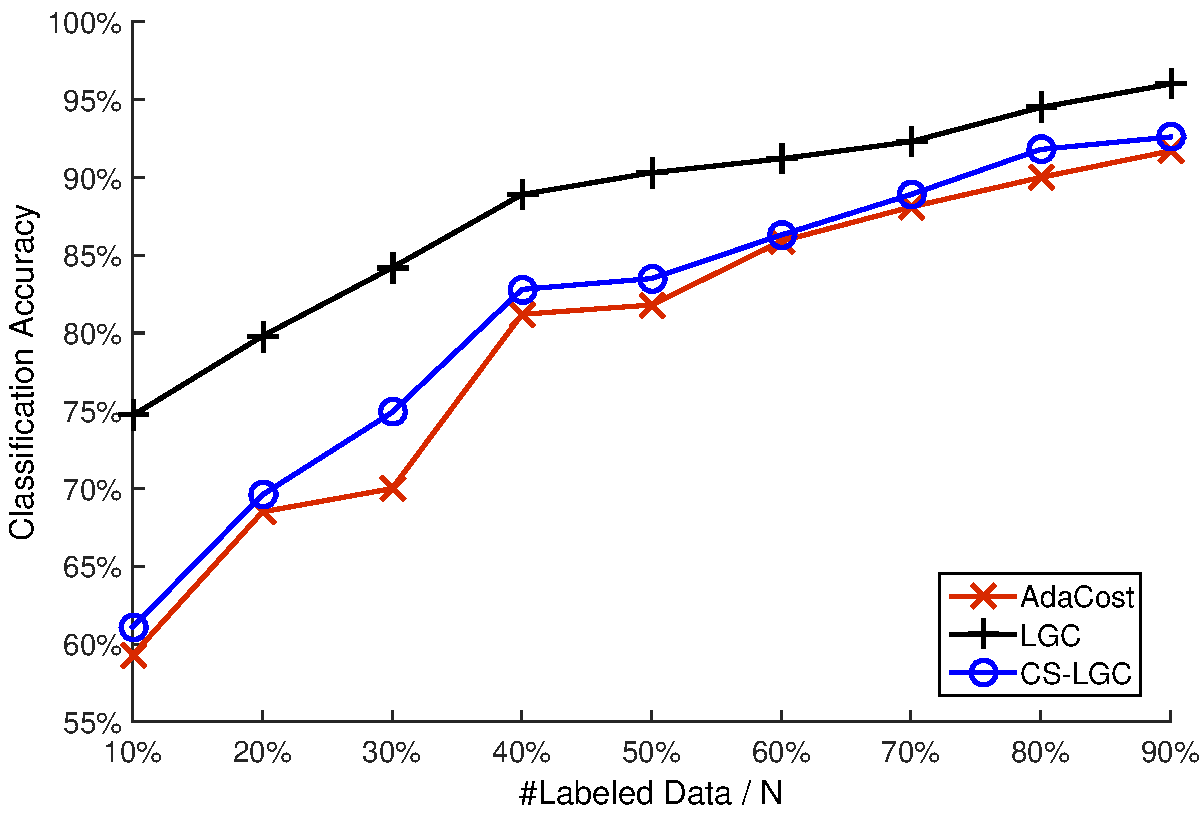
\includegraphics[width=\textwidth]{plot/fig2.pdf}
\caption{Global Classification Accuracy} \label{fig2}
\end{minipage}
\end{figure}

From Fig. \ref{fig1}, we can see, when the data size increases, the classification accuracies of three algorithm's high-cost data samples increase as well. However, CS-LGC and AdaCost can always achieve high level of accuracy and their average accuracies reach 92\%, which appears 7\% higher compared with LGC algorithm. This implies that CS-LGC and AdaCost pay more attention to the sample data of high-cost class, which shows their cost-sensitive feature. Nevertheless, when the percentage of the labeled data is lower than 50\%, AdaCost's accuracy fluctuates because of introduction of cost performance function, resulting in Boosting algorithm failing to converge to Bayesian decision. In addition, in Fig. \ref{fig1}, when the percentage of labeled data increases to 70\%, the classification accuracy of CS-LGC algorithm appears a slight decline, which is mainly attributed to the decrease of labeled data volume caused by cost update.

% \begin{figure}[H]
% 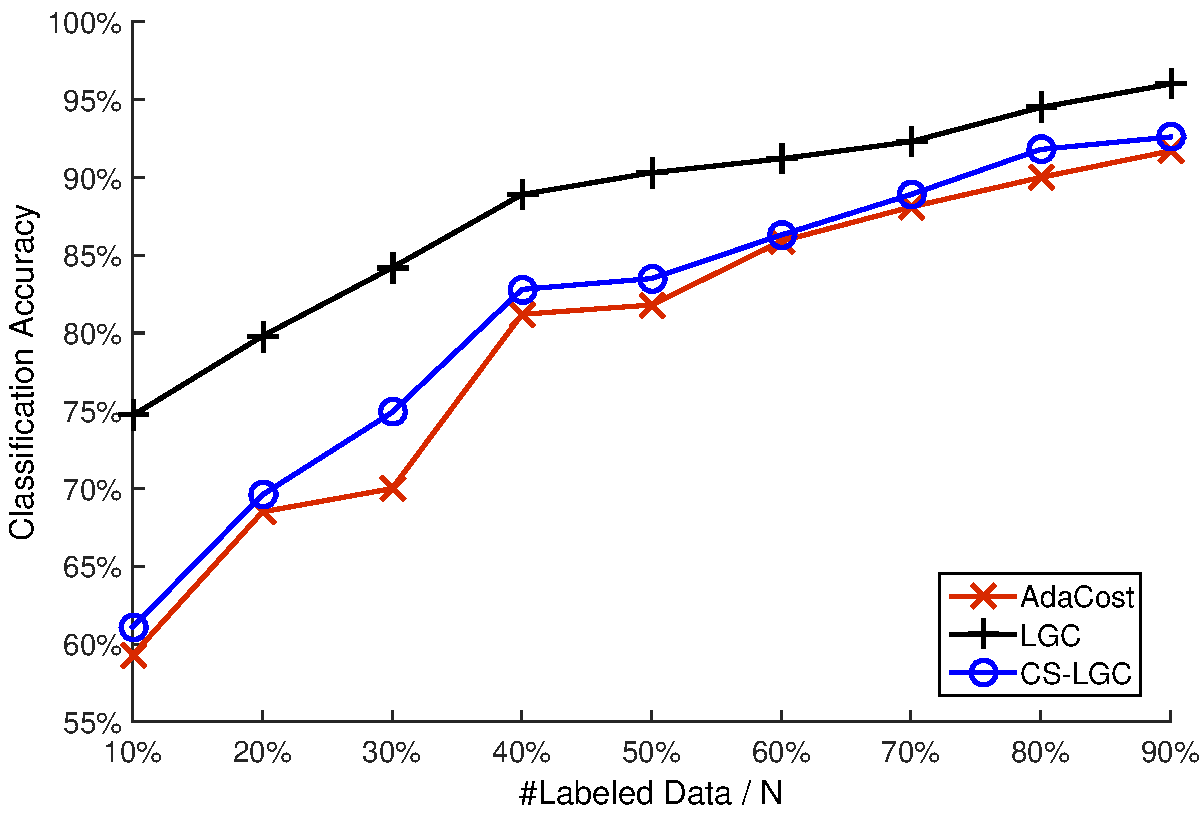
\includegraphics[width=\textwidth]{plot/fig2.pdf}
% \caption{Global Classification Accuracy} \label{fig2}
% \end{figure}
Fig. \ref{fig2} shows the curve of the global classification accuracy changing with the size of labeled data. In the figure, the average classification accuracy of LGC algorithm is about 90\%, 10\% higher than that of CS-LGC and AdaCost. It indicates that, cost-sensitive classification algorithm pays more attention on high cost class samples. Because the number of low-cost class samples is larger, the global classification accuracy of CS-LGC is lower than LGC. But the classification accuracy can still stay at an acceptable range, and with the increase of labeled data, the global classification accuracy goes up obviously. When the percentage of the labeled data is up to 90\%, the global classification accuracy of all three algorithm reach a higher level over 90\%. The global classification accuracy of CS-LGC is higher than AdaCost algorithm by about 2\% on average.

\begin{figure}[H]
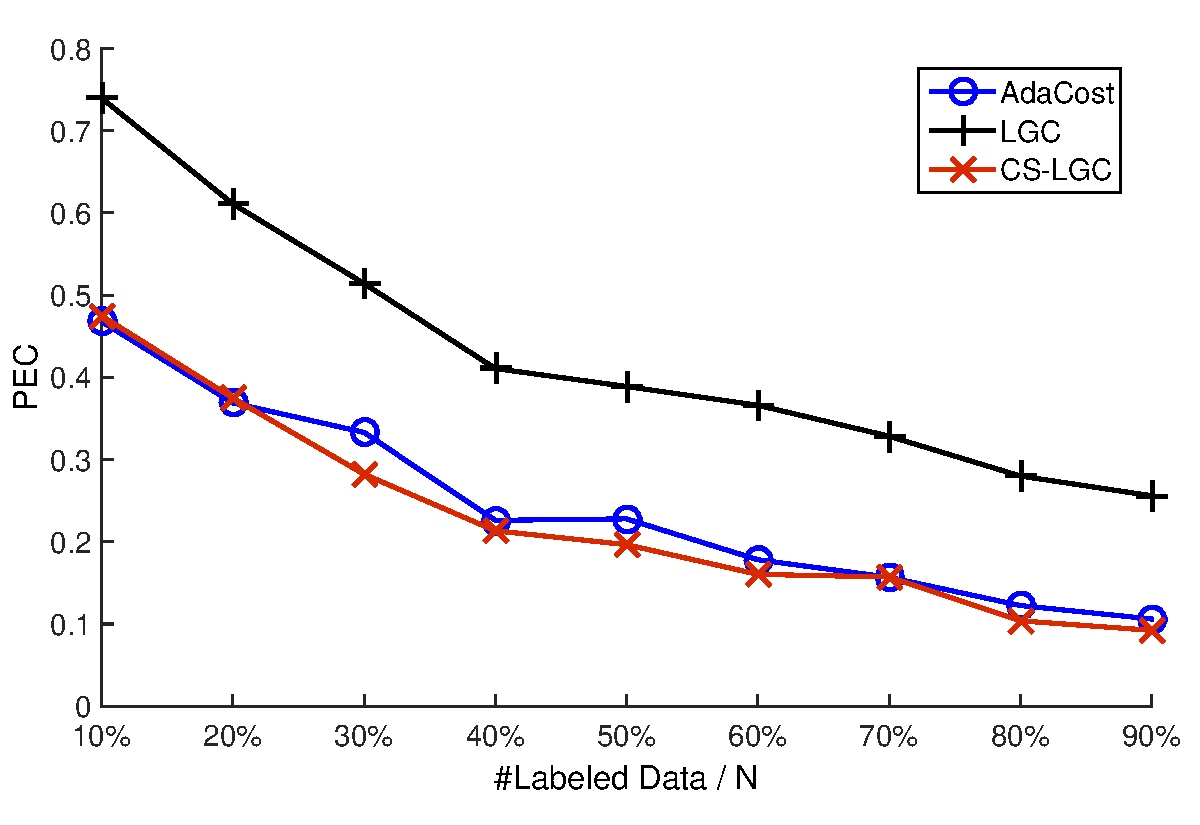
\includegraphics[width=\textwidth]{plot/fig3.pdf}
\caption{The Global Cost} \label{fig3}
\end{figure}
Fig. \ref{fig3} shows the global cost changing with the size of labeled data. In Fig. \ref{fig3}, the global costs of CS-LGC and AdaCost are obviously lower than LGC, by about 0.2 on average. We can know from both Fig. \ref{fig2} and Fig. \ref{fig3}, cost-sensitive classification sacrifices some classification accuracy, in exchange for a lower global cost, and CS-LGC performs best among the three.Besides, CS-LGC algorithm converges faster when the labeled data size increases, and the iteration time decreases, whose average value is between 10 and 20. 

In Summary, in the loan application problem, cost-sensitive classification algorithm pays more attention on high-cost class samples. By ensuring the low classification accuracy of high-cost class, it achieves the aim of reducing the global cost, and maintain global classification accuracy in the acceptable range.In conclusion, our CS-LGC algorithm performs best comprehensively.

\subsection{Breast Cancer Data Set}\label{subsec:exp2}
In the disease diagnosis problem, there is a higher cost for diagnosing patients with diseases as healthy, therefore, we denote the malignants as high-cost class (negative class). Fig. 4 through Fig.6 describe the LGC, CS-LGC, and AdaCost three methods' classification accuracy of high cost class. The global classification accuracy and global cost, which all vary with the number of labeled data in the figures.

\begin{figure}[H]
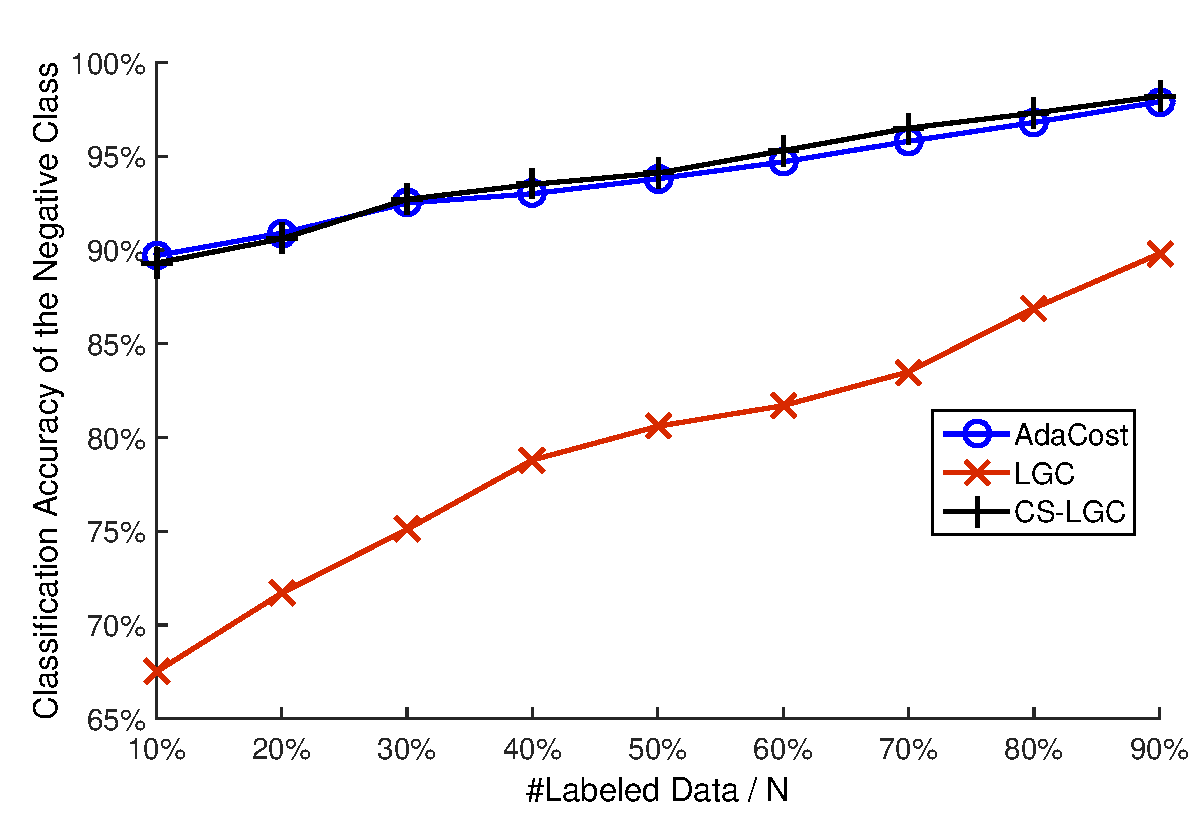
\includegraphics[width=\textwidth]{plot/fig4.pdf}
\caption{High-cost Class Classification Accuracy} \label{fig4}
\end{figure}

From Fig. \ref{fig4} we can see, the high-cost class classification accuracy of LGC algorithm is obviously lower than CS-LGC and AdaCost’s. Compared with the other two methods, It has the average accuracy lower by 10\%, yet still keeps above 70\%. It can be seen, CS-LGC and AdaCost pay more attention to high-cost class, but the high-cost class classification accuracy of CS-LGC algorithm is slightly higher than that of AdaCost algorithm.

\begin{figure}[H]
\begin{minipage}[t]{0.5\linewidth}
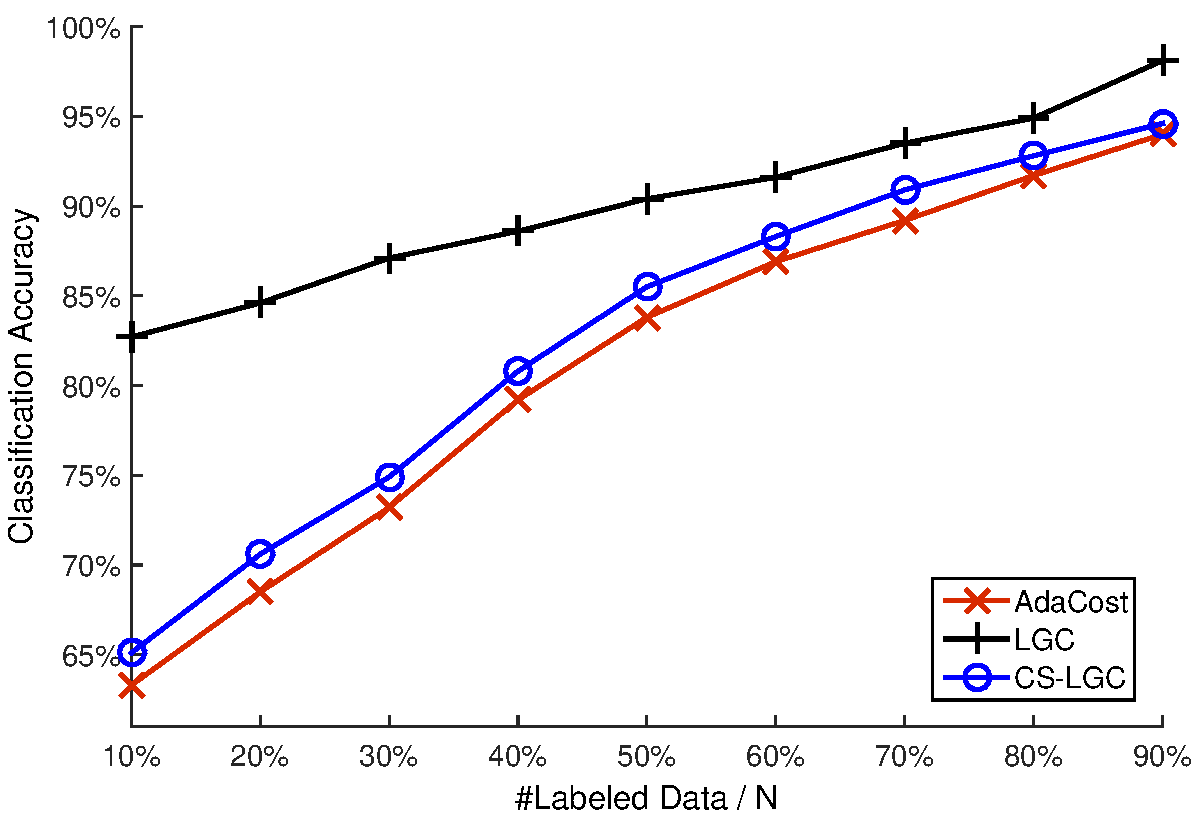
\includegraphics[width=\textwidth]{plot/fig5.pdf}
\caption{The Global Classification Accuracy} \label{fig5}
\end{minipage}
\begin{minipage}[t]{0.5\linewidth}
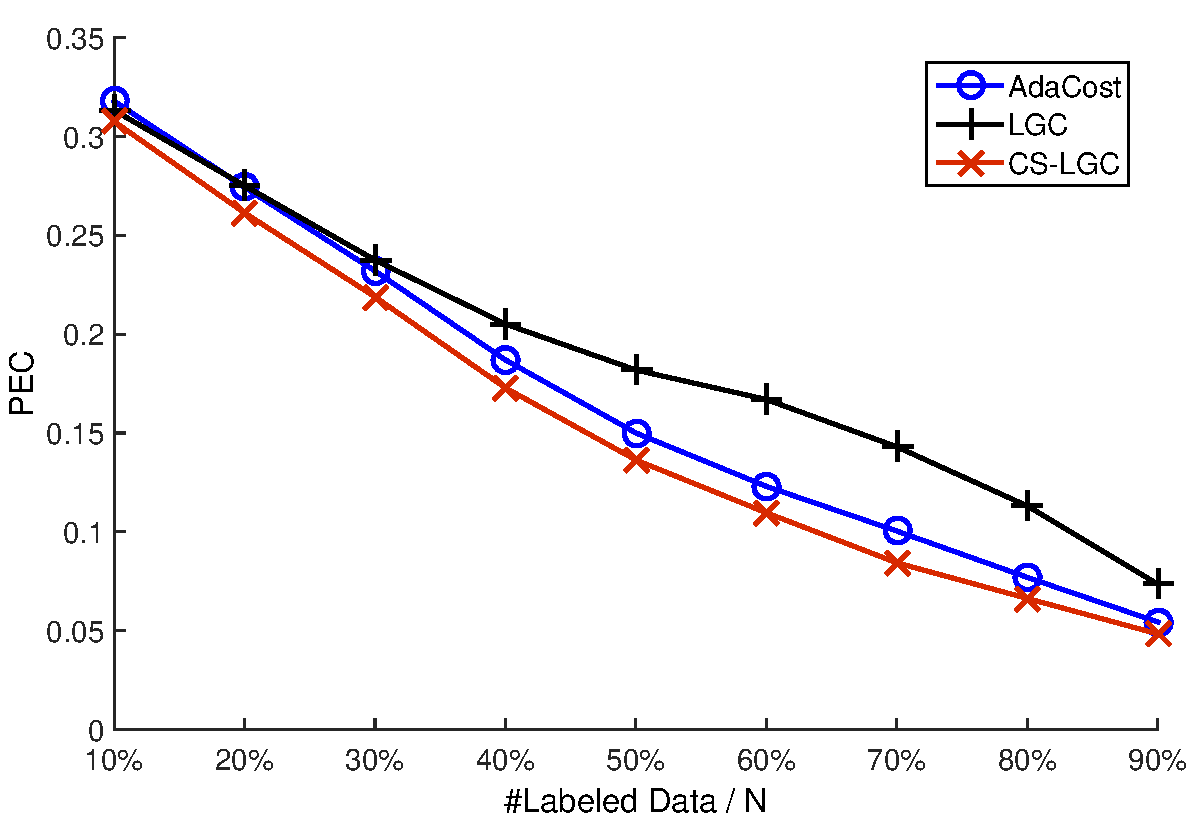
\includegraphics[width=\textwidth]{plot/fig6.pdf}
\caption{Average Cost of the Classifier} \label{fig6}
\end{minipage}
\end{figure}

Fig. \ref{fig5} shows that, with the increase of labeled data, the global classification accuracy of these three algorithms all increase accordingly, of which LGC algorithm has achieved a higher global classification accuracy by 9\% than the others on average. The global classification accuracy of CS-LGC and AdaCost increases faster with the increasing number of labeled data. When the percentage of the labeled data reaches about 70\%, the classification accuracy of these three algorithm reach the almost same level. The classification accuracy of CS-LGC is 2\% higher that of AdaCost on average.

And as it can be seen from Fig. \ref{fig6}, the global costs of this three algorithm show little difference, but the global cost of the CS-LGC algorithm is slightly better than the other two. Meanwhile, the global cost of LGC is higher than the other two algorithms by 5\% on average. Similarly, using this data set, CS-LGC can achieve convergence after only 10 times iteration on average.

As we can see from Fig. \ref{fig1}, Fig. \ref{fig2}, Fig. \ref{fig4} and
Fig. \ref{fig5}, when the portion of labeled data is little (less than 50\% in general), semi-supervision classification algorithm can reach a relatively high classification accuracy.

\subsection{The Analysis of CSS-LGC Algorithm Experiment}
We set three experiments to verify the performance of CSS-LGC method using the German Credit Data Set.

\begin{figure}[H]
\begin{minipage}[t]{0.5\linewidth}
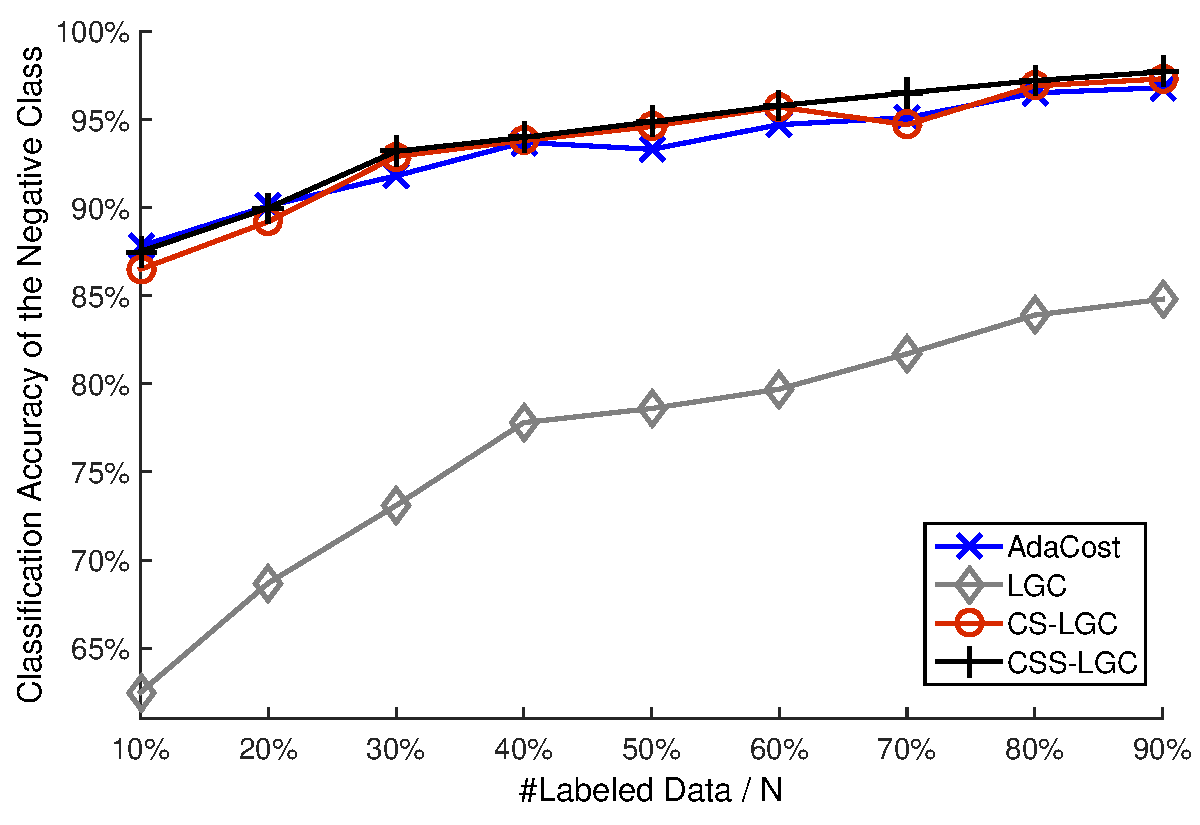
\includegraphics[width=\textwidth]{plot/fig7.pdf}
\caption{Changes in Classification Accuracy of Negative Class with Labeled Data Scale} \label{fig7}
\end{minipage}
\begin{minipage}[t]{0.5\linewidth}
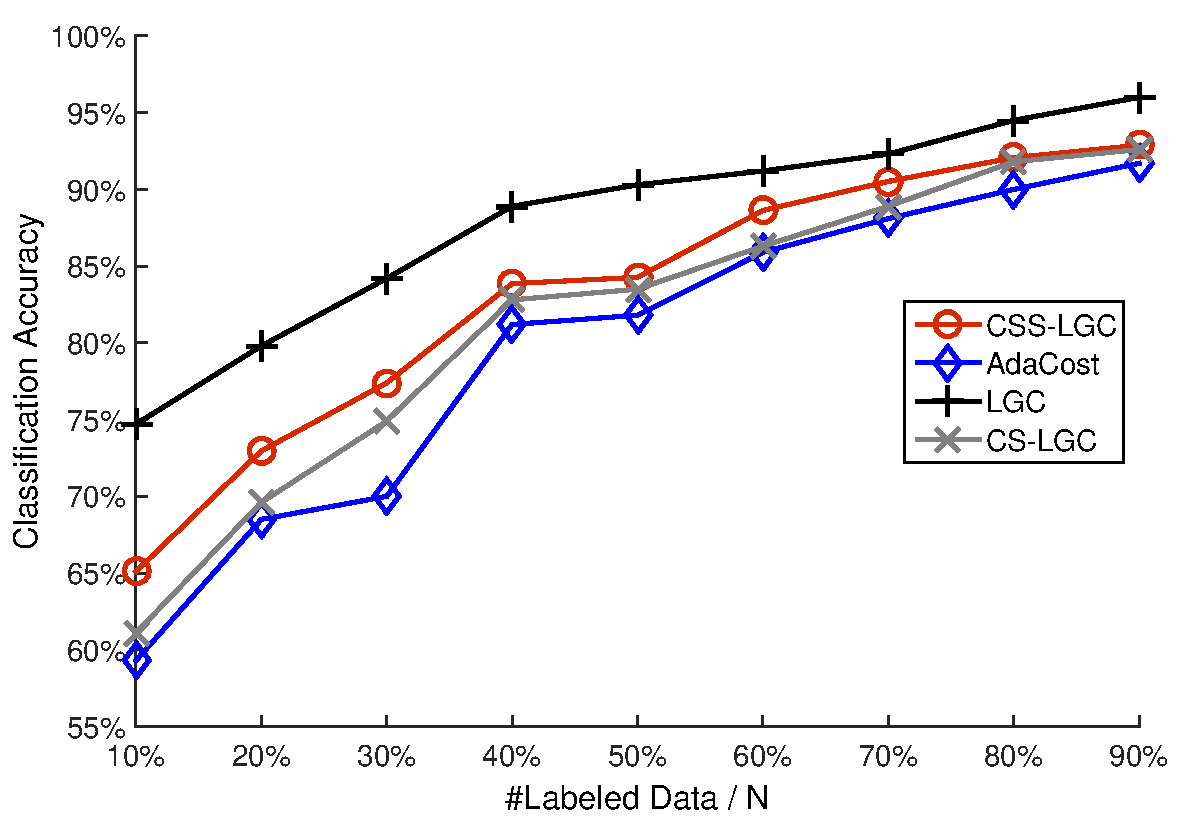
\includegraphics[width=\textwidth]{plot/fig8.pdf}
\caption{Changes in Classification Accuracy with Labeled Data Scale} \label{fig8}
\end{minipage}
\end{figure}

Fig. \ref{fig7} and Fig. \ref{fig8} show the four algorithms - LGC, CS-LGC, AdaCost and CSS-LGC algorithm's high-cost class classification accuracy and global classification accuracy, while Fig. \ref{fig9} describes global cost variation curve, when the labeled data scale increases from only 10\% to 90\% of the total data volume respectively.

\begin{figure}[h]
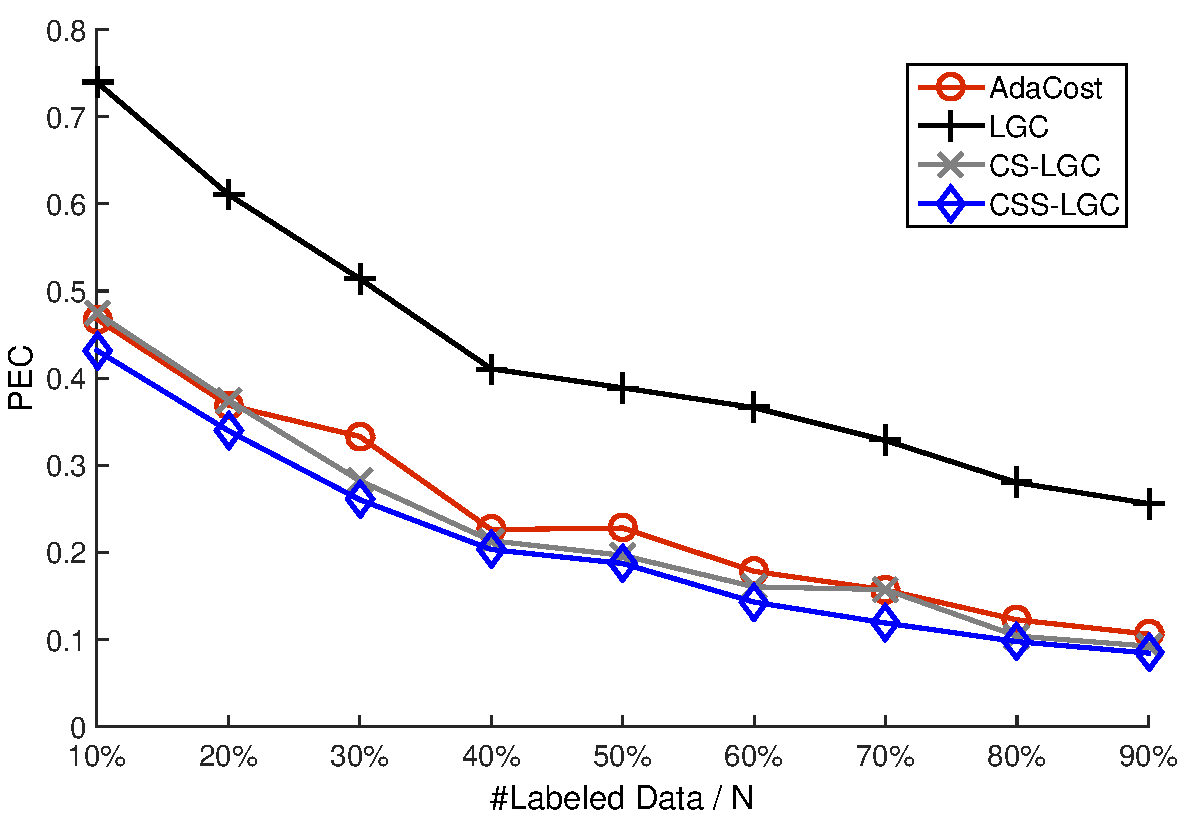
\includegraphics[width=\textwidth]{plot/fig9.pdf}
\caption{Changes in PEC with Labeled Data Scale} \label{fig9}
\end{figure}

From Fig. \ref{fig7}, Fig. \ref{fig8} and Fig. \ref{fig9}, we can see, in the initial stage of data set training, there is little difference between CSS-LGC and CS-LGC algorithm. That is because in the beginning, the little amount of minority class samples do not work in the data set. At this time, there are enough unlabeled data for minority class can be chosen. But with the proceeding of the training, the number of unlabeled data is declining. Then the weakness of minority class data will be evident for the selection of unlabeled data using CS-LGC algorithm, which does not take the number of minority class samples into account.That will cause error accumulation, and undermine performance of
CS-LGC algorithm. However, when the unlabeled data of minority class is trained by CSS-LGC algorithm, SMOTE algorithm introduced in works. And with the method of synthesizing, some virtual unlabeled data of weak minority are created. Then unlabeled data of minority class are continuously generated until conditions are met by comparison, which can be accepted by CS-LGC algorithm.


\section{Conclusions}

In this paper, we proposed CS-LGC algorithm that introduced cost sensitivity into classic semi-supervised classification algorithm based on AdaBoost method, and obtained better performance
global classifier in the way of weighted voting for weak classifiers.

We take into account the defects that may be caused by imbalanced data set, improved CS-LGC
algorithm and proposed CSS-LGC algorithm. In semi-supervised learning, CSS-LGC algorithm makes full use of a large number of unlabeled data. Considering heterogeneous distribution of misclassification
cost in real life, cost sensitivity is introduced into LGC algorithm. In the process of label matrix update, CSS-LGC algorithm improves its comprehensive performance and generalization using SMOTE method that can eliminate the effect of imbalanced data sets. Therefore, CSS-LGC algorithm is practical and instructive in solving real-life problems.

However, CSS-LGC algorithm's performance will be compromised because similarity computation will appear more times and take more time to find out required unlabeled data in the Rescale process. Thus in our future work, we plan to simplify the calculation of average similarity, optimize SMOTE method and improve overall performance of CSS-LGC further.
% \section{Section title}
% \label{sec:1}
%Text with citations  and %\cite{urner2011access} \cite{zhou2010semi} \cite{zhu2009introduction} \cite{budvytis2010label} \cite{zhu2003semi} \cite{zhou2004learning} \cite{gao2011active} \cite{elkan2001foundations} \cite{zhou2010multi} \cite{domingos1999metacost} \cite{khoshgoftaar2011comparing} \cite{fan1999adacost} \cite{jin2010multi} \cite{qin2008cost} \cite{liu2006influence} \cite{seiffert2008comparative} \cite{bache2013uci} \cite{germandata}
% \subsection{Subsection title}
% \label{sec:2}
% as required. Don't forget to give each section
% and subsection a unique label (see Sect.~\ref{sec:1}).graphystyle{spbasic}      % basic style, author-year citations
%\bibliographystyle{spmpsci}      % mathematics and physical sciences
%\bibliographystyle{spphys}       % APS-like style for physics
%\bibliography{}   % name your BibTeX data base
\bibliographystyle{ieeetr}
\bibliography{myref}

% Non-BibTeX users please use
\end{document}
% end of file template.tex

